\section{Kenapa kita membutuhkan komputasi parallel?}

Pertumbuhan daya komputasi yang disediakan oleh komputer modern telah menghasilkan masalah komputasi yang semakin kompleks dalam jangka waktu yang relatif singkat. Sampai awal 2000-an, kompleksitas ditangani dengan meningkatkan jumlah transistor serta frekuensi clock dari sistem prosesor tunggal, yang mencapai puncak 3,5-4 GHz. Namun, peningkatan jumlah transistor menyebabkan peningkatan eksponensial dari daya yang dihabiskan oleh prosesor itu sendiri. Pada dasarnya, ada, oleh karena itu, keterbatasan fisik yang mencegah peningkatan lebih lanjut dalam kinerja sistem prosesor tunggal.
\noindent
Untuk alasan ini, dalam beberapa tahun terakhir, produsen mikroprosesor memusatkan perhatian mereka pada sistem multi-core. Ini didasarkan pada inti dari beberapa prosesor fisik yang berbagi memori yang sama, sehingga dengan melewatkan masalah daya yang hilang yang dijelaskan sebelumnya. Dalam beberapa tahun terakhir, sistem quad-core dan octa-core juga telah menjadi standar pada konfigurasi desktop dan laptop normal.
\noindent
Di sisi lain, perubahan signifikan dalam perangkat keras juga menghasilkan evolusi struktur perangkat lunak, yang selalu dirancang untuk dieksekusi secara berurutan pada satu prosesor. Untuk mengambil keuntungan dari sumber daya komputasi yang lebih besar yang tersedia dengan meningkatkan jumlah prosesor, perangkat lunak yang ada harus dirancang ulang dalam bentuk yang sesuai dengan struktur paralel CPU, sehingga dapat memperoleh efisiensi yang lebih besar melalui eksekusi simultan dari unit tunggal dari beberapa bagian dari program yang sama.

\section{Taksonomi Flynn}
Taksonomi Flynn adalah sistem untuk mengklasifikasikan arsitektur komputer. Ini didasarkan pada dua konsep utama:

\begin{enumerate}
	\item Instruction flow: Suatu sistem dengan n CPU memiliki n penghitung program dan, oleh karena itu, n instruksi mengalir. Ini sesuai dengan penghitung program.
	\item Data flow: Program yang menghitung fungsi pada daftar data memiliki aliran data. Program yang menghitung fungsi yang sama pada beberapa daftar data yang berbeda memiliki lebih banyak aliran data. Ini terdiri dari seperangkat operan.
\end{enumerate}

\noindent
Karena instruksi dan aliran data bersifat independen, ada empat kategori mesin paralel: Single Instruction Single Data (SISD), Single Instruction Multiple Data (SIMD), Multiple Instruction Single Data (MISD), and Multiple Instruction Multiple Data (MIMD):

\begin{figure}[H]
	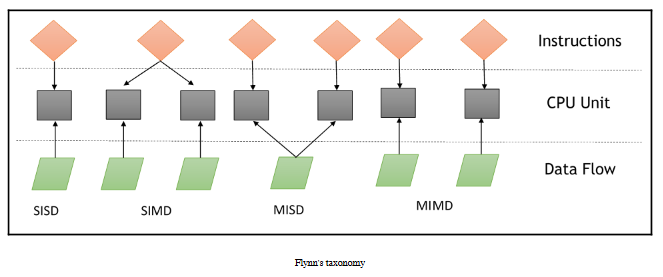
\includegraphics[width=4cm]{figures/kelompok2/chapter1/1.png}
	\centering
	\caption{Flynn.}
\end{figure}

\subsection{Single Instruction Single Data (SISD)}
Sistem komputasi SISD seperti mesin von Neumann, yang merupakan mesin uniprocessor. Seperti yang Anda lihat dalam diagram taksonomi Flynn, ia menjalankan instruksi tunggal yang beroperasi pada aliran data tunggal. Di SISD, instruksi mesin diproses secara berurutan.

\noindent
Dalam siklus clock, CPU menjalankan operasi berikut:

\begin{enumerate}
	\item Fetch: CPU mengambil data dan instruksi dari area memori, yang disebut register.
	\item Decode: CPU menerjemahkan instruksi.
	\item Execute: Instruksi dilakukan pada data. Hasil operasi disimpan dalam register lain.
\end{enumerate}

\noindent
Setelah tahap eksekusi selesai, CPU menetapkan dirinya untuk memulai siklus CPU lain:

\begin{figure}[H]
	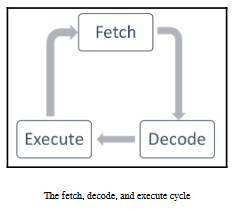
\includegraphics[width=4cm]{figures/kelompok2/chapter1/2.png}
	\centering
	\caption{SISD.}
\end{figure}

\noindent
Algoritma yang berjalan pada komputer jenis ini bersifat berurutan (atau serial) karena tidak mengandung paralelisme. Contoh komputer SISD adalah sistem perangkat keras dengan satu CPU.

\noindent
Elemen utama dari arsitektur ini (yaitu, arsitektur von Neumann) adalah sebagai berikut:

\begin{enumerate}
	\item Central memori unit: Ini digunakan untuk menyimpan instruksi dan data program.
	\item CPU: Ini digunakan untuk mendapatkan instruksi dan / atau data dari unit memori, yang menerjemahkan instruksi dan secara berurutan mengimplementasikannya.
	\item The I/O system: Ini mengacu pada data input dan output dari program.
\end{enumerate}

\noindent
Komputer prosesor tunggal konvensional diklasifikasikan sebagai sistem SISD:

\begin{figure}[H]
	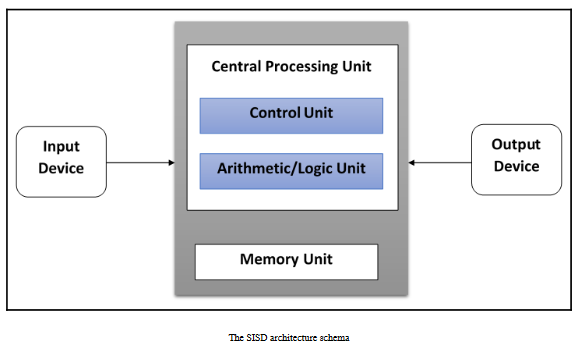
\includegraphics[width=4cm]{figures/kelompok2/chapter1/3.png}
	\centering
	\caption{Algoritma SISD.}
\end{figure}

\noindent
Diagram berikut secara khusus menunjukkan area mana dari CPU yang digunakan pada tahap pengambilan, dekode, dan eksekusi:

\begin{figure}[H]
	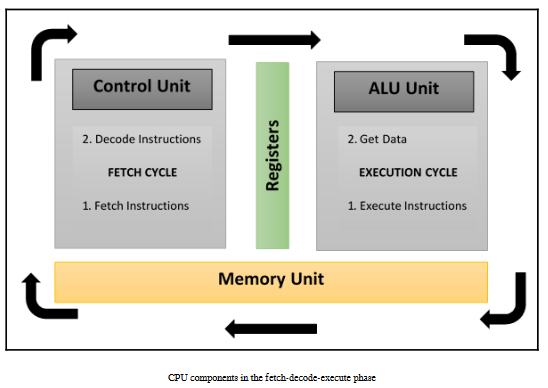
\includegraphics[width=4cm]{figures/kelompok2/chapter1/4.png}
	\centering
	\caption{Area Fetch CPU.}
\end{figure}

\subsection{MISD}
\textit{Multiple Instruction Single Data} \textbf{(MISD)}. Dalam model ini, prosesor, masing-masing dengan unit kontrol mereka sendiri, berbagi unit memori tunggal. Dalam setiap siklus clock, data yang diterima dari memori diproses oleh semua prosesor secara bersamaan, masing-masing sesuai dengan instruksi yang diterima dari unit kontrol. Dalam hal ini, paralelisme (paralelisme tingkat instruksi) diperoleh dengan melakukan beberapa operasi pada bagian data yang sama. Jenis masalah yang dapat dipecahkan secara efisien dalam arsitektur ini agak istimewa, seperti enkripsi data. Untuk alasan ini, komputer MISD belum menemukan ruang di sektor komersial. Komputer MISD lebih dari satu latihan intelektual daripada konfigurasi praktis

\subsection{SIMD}
\textit{Single Instruction Multiple Data} \textbf{(SIMD)}. Sebuah SIMD komputer terdiri dari n prosesor yang identik, masing-masing dengan memori lokal mereka sendiri, di mana dimungkinkan untuk menyimpan data. Semua prosesor bekerja di bawah kendali aliran instruksi tunggal. Selain itu, ada n data stream, satu untuk setiap prosesor. Prosesor bekerja secara simultan pada setiap langkah dan menjalankan instruksi yang sama, tetapi pada elemen data yang berbeda. Ini adalah contoh dari data tingkat paralelisme.
SIMD arsitektur jauh lebih fleksibel daripada arsitektur MISD. Banyak masalah yang mencakup berbagai macam aplikasi dapat diselesaikan dengan algoritma paralel pada komputer SIMD. Fitur lain yang menarik adalah bahwa algoritma untuk komputer ini relatif mudah untuk merancang, menganalisis, dan menerapkan. pembatasan adalah bahwa hanya masalah yang dapat dibagi menjadi beberapa submasalah (yang semuanya identik, yang masing-masing kemudian akan diselesaikan secara simultan melalui set instruksi yang sama) dapat diatasi dengan komputer SIMD.
\subsection{MIMD}
\textit{Multiple Instruction Multiple Data} \textbf{MIMD}. kelas ini merupakan kelas umum dan paling kuat, menurut klasifikasi Flynn. Ini mengandung prosesor, instruksi stream, dan data stream. Setiap prosesor memiliki satuan sendiri kontrol dan memori lokal, yang membuat MIMD arsitektur lebih komputasi kuat dari arsitektur SIMD.
Setiap prosesor beroperasi di bawah kendali aliran instruksi yang dikeluarkan oleh unit kontrol sendiri. Oleh karena itu, prosesor berpotensi dapat menjalankan program yang berbeda dengan data yang berbeda, yang memungkinkan mereka untuk memecahkan submasalah yang berbeda dan dapat menjadi bagian dari masalah yang lebih besar tunggal. Dalam MIMD, arsitektur dicapai dengan bantuan tingkat paralelisme dengan benang dan / atau proses. Ini juga berarti bahwa prosesor biasanya beroperasi asynchronous.

Saat ini, arsitektur ini diterapkan untuk banyak PC, superkomputer, dan jaringan komputer. Namun, ada counter yang perlu Anda pertimbangkan: algoritma asynchronous sulit untuk merancang, menganalisis, dan menerapkan:

\begin{figure}[H]
	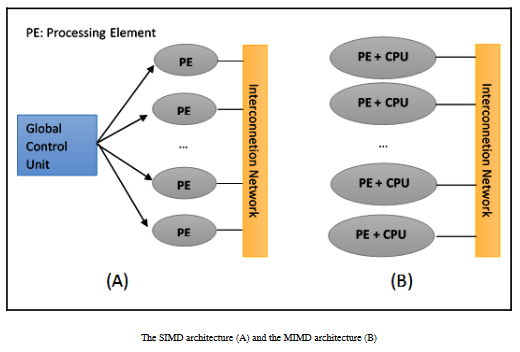
\includegraphics[width=4cm]{figures/kelompok2/chapter1/5.png}
	\centering
	\caption{MIMD.}
\end{figure}

\section{Organisasi Memori}
Aspek lain yang perlu kita pertimbangkan dalam rangka untuk mengevaluasi arsitektur paralel organisasi memori, atau lebih tepatnya, cara di mana data yang diakses. Tidak peduli seberapa cepat unit pengolahan, jika memori tidak dapat mempertahankan dan memberikan petunjuk dan data pada kecepatan yang cukup, maka tidak akan ada peningkatan kinerja. Masalah utama yang kita butuhkan untuk mengatasi untuk membuat waktu respon dari memori yang kompatibel dengan kecepatan prosesor adalah memori waktu siklus, yang didefinisikan sebagai waktu yang telah berlalu antara dua operasi berturut-turut. Waktu siklus prosesor biasanya lebih singkat daripada waktu siklus memori.

Ketika prosesor memulai transfer ke atau dari memori, sumber daya prosesor akan tetap diduduki untuk seluruh durasi siklus memori; Selanjutnya, selama periode ini, tidak ada perangkat lain (misalnya, I / O controller, prosesor, atau bahkan prosesor yang membuat permintaan) akan dapat menggunakan memori karena transfer berlangsung:
Masalahnya terjadi ketika prosesor memodifikasi data yang disimpan dalam sistem memori itu secara bersamaan digunakan oleh prosesor lain. Nilai baru akan lulus dari cache prosesor yang telah diubah ke memori bersama. Namun kemudian, itu juga harus diteruskan ke semua prosesor lainnya, sehingga mereka tidak bekerja dengan nilai usang. Masalahnya adalah dikenal sebagai masalah koherensi cache — kasus khusus dari masalah memori konsistensi, yang memerlukan implementasi perangkat keras yang dapat menangani masalah konkurensi dan sinkronisasi, mirip dengan pemrograman thread.

Fitur utama dari sistem memori bersama adalah sebagai berikut: Memori sama untuk semua prosesor. Misalnya, semua prosesor terkait dengan struktur data yang sama akan bekerja dengan memori logis yang sama alamat, sehingga mengakses lokasi memori yang sama. Sinkronisasi diperoleh dengan membaca tugas berbagai prosesor dan memungkinkan memori bersama. Bahkan, prosesor hanya dapat mengakses satu memori pada suatu waktu. Lokasi memori bersama tidak boleh diubah dari tugas sementara tugas lain mengaksesnya. Berbagi data antar tugas dengan cepat. Waktu yang dibutuhkan untuk berkomunikasi adalah waktu yang diperlukan salah satu dari mereka untuk membaca satu lokasi (tergantung pada kecepatan akses memori).

Akses memori dalam sistem memori bersama adalah sebagai berikut :
\begin{enumerate}
\item Akses memori dalam sistem memori bersama adalah sebagai berikut: 
\item Uniform Memory Access (UMA): Karakteristik mendasar dari sistem ini adalah waktu akses ke memori yang konstan untuk setiap prosesor dan untuk apa saja area memori. Untuk alasan ini, sistem ini juga disebut Simetris Multiprosesor (SMP). Mereka relatif sederhana untuk diterapkan, tetapi tidak terlalu terukur. Coder bertanggung jawab atas pengelolaan sinkronisasi oleh memasukkan kontrol yang sesuai, semaphores, mengunci, dan lainnya di program itu mengelola sumber daya
\item Non-Uniform Memory Access (NUMA): Arsitektur ini membagi memori ke area akses berkecepatan tinggi yang ditugaskan untuk setiap prosesor, dan juga, a area umum untuk pertukaran data, dengan akses yang lebih lambat. Sistem ini juga disebut sistem Distributed Shared Memory (DSM). Mereka sangat scalable, tetapi kompleks untuk dikembangkan. 
\item Tidak Ada Akses Memori Jarak Jauh (NoRMA): Memori didistribusikan secara fisik di antara prosesor (memori lokal). Semua kenangan lokal bersifat pribadi dan bisa hanya mengakses prosesor lokal. Komunikasi antara prosesor adalah melalui protokol komunikasi yang digunakan untuk bertukar pesan, yaitu dikenal sebagai protokol penyampaian pesan.
\item Cache-Only Memory Arsitektur (Koma): Sistem ini dilengkapi dengan kenangan hanya cache. Sementara menganalisis arsitektur NUMA, itu menyadari bahwa arsitektur ini terus salinan lokal dari data dalam cache dan data ini disimpan sebagai duplikat dalam memori utama. Arsitektur ini menghilangkan duplikat dan membuat hanya kenangan cache; memori didistribusikan secara fisik antara prosesor (memori lokal). Semua kenangan lokal pribadi dan hanya dapat mengakses prosesor lokal. Komunikasi antara prosesor juga melalui protokol pesan-lewat.
\end{enumerate}
\begin{figure}[H]
	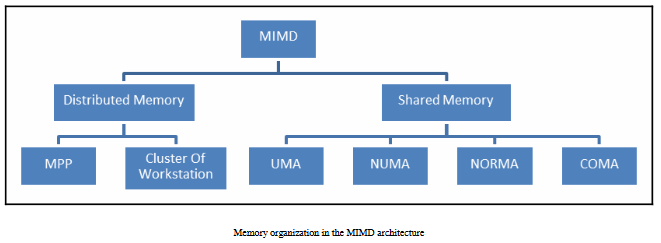
\includegraphics[width=4cm]{figures/kelompok2/chapter1/6.png}
	\centering
	\caption{Memory Organization.}
\end{figure}

\subsection{Shared Memory}

\begin{figure}[H]
	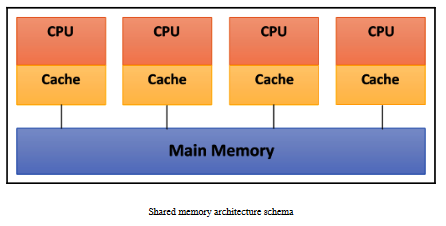
\includegraphics[width=4cm]{figures/kelompok2/chapter1/7.png}
	\centering
	\caption{Shared Memory.}
\end{figure}

\subsection{Distributed Memory}
 Dalam sistem dengan memori terdistribusi, memori dikaitkan dengan masing-masing prosesor dan sebuah prosesor hanya mampu mengatasi memori sendiri. Beberapa penulis menyebut jenis sistem sebagai multicomputer suatu, mencerminkan fakta bahwa unsur-unsur dari sistem ini adalah, sendiri, sistem yang kecil dan lengkap dari prosesor dan memori, seperti yang Anda lihat pada diagram berikut:
\begin{figure}[H]
	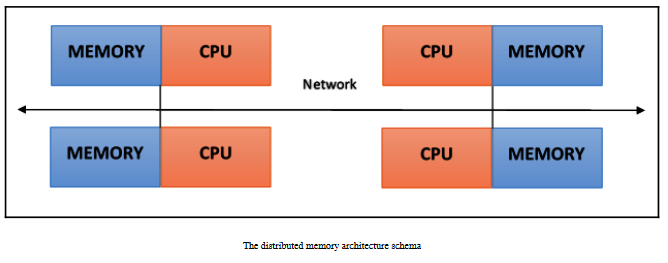
\includegraphics[width=4cm]{figures/kelompok2/chapter1/8.png}
	\centering
	\caption{Distributed Memory.}
\end{figure}
\noindent
organisasi semacam ini memiliki beberapa keunggulan:

\begin{enumerate}
	\item Tidak ada konflik di tingkat bus komunikasi atau switch. Setiap prosesor dapat menggunakan bandwidth penuh memori lokal mereka sendiri tanpa campur tangan dari prosesor lainnya.
	\item Kurangnya sarana bus umum yang tidak ada batas intrinsik untuk jumlah prosesor. Ukuran sistem ini hanya dibatasi oleh jaringan yang digunakan untuk menghubungkan prosesor.
	\item Tidak ada masalah dengan koherensi cache. Setiap prosesor bertanggung jawab untuk data sendiri dan tidak harus khawatir tentang upgrade salinan apapun.

Kerugian utama adalah bahwa komunikasi antara prosesor lebih sulit untuk menerapkan. Jika prosesor membutuhkan data dalam memori prosesor lain, maka dua prosesor tidak harus selalu bertukar pesan melalui protokol pesan-lewat. Ini memperkenalkan dua sumber perlambatan: untuk membangun dan mengirim pesan dari satu prosesor ke yang lain membutuhkan waktu, dan juga, setiap prosesor harus dihentikan untuk mengelola pesan yang diterima dari prosesor lainnya. Sebuah program yang dirancang untuk bekerja pada mesin memori terdistribusi harus diselenggarakan sebagai satu set tugas independen yang berkomunikasi melaluipesan:
\end{enumerate}

\begin{figure}[H]
	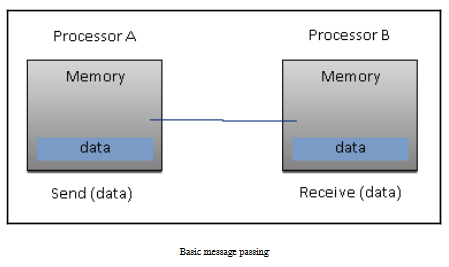
\includegraphics[width=4cm]{figures/kelompok2/chapter1/9.png}
	\centering
	\caption{Distributed Memory 2.}
\end{figure}

\noindent
Fitur utama dari sistem memori terdistribusi adalah sebagai berikut:

\begin{enumerate}
	\item Memori secara fisik didistribusikan antara prosesor; setiap memori lokal secara langsung dapat diakses hanya dengan prosesor.
	\item Sinkronisasi dicapai dengan memindahkan data (bahkan jika itu hanya pesan itu sendiri) antara prosesor (komunikasi).
	\item Subdivisi data dalam kenangan lokal mempengaruhi kinerja mesin-adalah penting untuk membuat subdivisi akurat, sehingga dapat meminimalkan komunikasi antara CPU. Selain itu, prosesor yang koordinat operasi ini dekomposisi dan komposisi harus berkomunikasi secara efektif dengan prosesor yang beroperasi pada bagian-bagian individu dari struktur data.
         \item Protokol message-passing digunakan sehingga CPU dapat berkomunikasi satu sama lain melalui pertukaran paket data. Pesan adalah unit diskrit informasi, dalam arti bahwa mereka memiliki identitas yang jelas, sehingga selalu mungkin untuk membedakan mereka dari satu sama lain.


\subsection{MPP}
mesin MPP terdiri dari ratusan prosesor (yang dapat sebagai besar sebagai ratusan ribu prosesor di beberapa mesin) yang terhubung oleh jaringan komunikasi. Komputer tercepat di dunia didasarkan pada arsitektur ini; beberapa contoh dari sistem arsitektur ini Earth Simulator, Blue Gene, ASCI White, ASCI Merah, dan ASCI Purple dan Red Storm-storm.

\subsection{Clusters of Workstations}
\item Sistem pengolahan didasarkan pada komputer klasik yang dihubungkan oleh jaringan komunikasi. cluster komputasi jatuh ke dalam klasifikasi ini.
\item Dalam arsitektur cluster, kita mendefinisikan node sebagai unit komputasi tunggal yang mengambil bagian dalam cluster. Untuk pengguna, cluster sepenuhnya transparan-semua perangkat keras dan perangkat lunak kompleksitas bertopeng dan data dan aplikasi yang dibuat dapat diakses seolah-olah mereka semua dari node tunggal.
\noindent Di sini, kami telah mengidentifikasi tiga jenis kelompok:
\item Gagal-lebih klaster: Dalam hal ini, kegiatan node terus dipantau, dan ketika salah satu berhenti bekerja, komputer lain mengambil alih jawab kegiatan tersebut. Tujuannya adalah untuk memastikan layanan terus menerus karena redundansi dari arsitektur yang baik.
\item Load balancing klaster: Dalam sistem ini, permintaan pekerjaan dikirim ke node yang memiliki kurang aktivitas. waktu Memastikan bahwa kurang ini diambil untuk memproses pekerjaan.
\item Kinerja tinggi komputasi klaster: Dalam hal ini, setiap node dikonfigurasi untuk memberikan kinerja yang sangat tinggi. Proses ini juga dibagi menjadi beberapa pekerjaan di beberapa node. Pekerjaan yang diparalelkan dan akan didistribusikan ke mesin yang berbeda.




\subsection{Heterogeneous Architectures}
Pengenalan akselerator GPU di dunia homogen superkomputer telah mengubah sifat bagaimana superkomputer keduanya digunakan dan diprogram sekarang. Meskipun kinerja tinggi yang ditawarkan oleh GPU, mereka tidak dapat dianggap sebagai unit pengolahan otonom karena mereka harus selalu disertai dengan kombinasi CPU. Paradigma pemrograman, karena itu, adalah sangat sederhana: CPU mengambil kendali dan hitungan secara serial, menetapkan tugas untuk akselerator grafis yang, komputasi, sangat mahal dan memiliki tingkat tinggi paralelisme yang baik.
\item Komunikasi antara CPU dan GPU dapat berlangsung, tidak hanya melalui penggunaan bus berkecepatan tinggi tetapi juga melalui berbagi satu daerah memori untuk memori fisik atau virtual. Bahkan, dalam kasus di mana kedua perangkat tidak dilengkapi dengan area memori mereka sendiri, adalah mungkin untuk mengacu pada area memori umum menggunakan perpustakaan software yang disediakan oleh berbagai model pemrograman, seperti CUDA dan OpenCL.
\item arsitektur ini disebut arsitektur heterogen, dimana aplikasi dapat membuat struktur data dalam ruang alamat tunggal dan mengirim pekerjaan ke perangkat keras, yang sesuai untuk resolusi tugas. Beberapa tugas pengolahan dapat beroperasi dengan aman di daerah yang sama untuk menghindari masalah konsistensi data, berkat operasi atom.
\item Jadi, terlepas dari kenyataan bahwa CPU dan GPU tampaknya tidak bekerja secara efisien bersama, dengan penggunaan arsitektur baru ini, kami dapat mengoptimalkan interaksi mereka dengan, dan kinerja, aplikasi paralel:



\begin{figure}[H]
	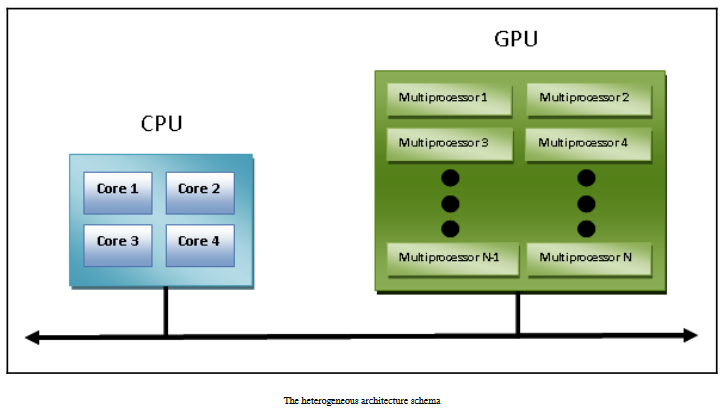
\includegraphics[width=4cm]{figures/kelompok2/chapter1/10.png}
	\centering
	\caption{Architectures.}
\end{figure}